\chapter{基于邻边卷积网络的复合物筛选模型}
\label{chapter:EdgeConv}

本章首先介绍了生物数据对复合物预测的重要性,介绍了生物数据在蛋白质相互作用网络中的邻边嵌入。同时介绍了基于邻边嵌入的相关图卷积算法,并提出了基于邻边卷积网络的复合物筛选模型。最后针对该模型进行了相关的对比实验并分析了实验结果。

\section{引言}
\label{section:EdgeConv:Put}

已有方法已经充分表明,在PPI网络中进行蛋白质复合物预测不仅仅是一个图论中的聚簇发现问题,更是一个信息融合问题。无论是加权网络方法、核心附属结构预测方法,都致力于最大程度的利用生物学信息进行辅助预测。

而已有的算法通常将生物学信息,包括GO功能注释、拓扑域、亚细胞定位等转换为蛋白质之间的相似性数据,即映射为邻边数据。已有的基于加权图的复合物预测算法是将邻边特征映射到固定的权重计算公式中,相较于基于无权图的算法,其预测复合物的质量有较好的提升,说明邻边数据在复合物预测领域具有一定的重要性。

然而,硬编码的过程只能将丰富的生物数据进行简单的映射,无法做到对生物数据的高维抽象。
目前该研究领域也尚未出现对邻边特征进行高维非线性抽象的算法。
基于以上前提,本文提出了利用生物特征基于邻边卷积网络的复合物局部子图分类模型。

\section{邻边卷积网络介绍}
\label{section:EdgeConv:intro}

邻边卷积网络\cite{wang_dynamic_2019}(EdgeBase Convolution)由点云学习领域提出,是一种基于邻边做特征转换以及特征聚合的方法。点云学习指的是使用计算机的方法学习与分析空间中独立数据点的集合,数据点的信息包括坐标、颜色、分类、强度值等等信息,数据点在空间中的集合状态即为点云。点云学习的任务是对点云数据做分割、物体识别等等。

在点云任务中,会与待更新结点i周围的K个最近邻居建立连边,基于连边做特征更新,然后所有的连边特征汇聚到一起作为结点的新特征。连边特征更新的过程中会考虑源点与汇点的信息流动,其具体的过程如图\ref{fig:EdgeConv/main}所示。
\begin{figure}[htbp]
    \centering
    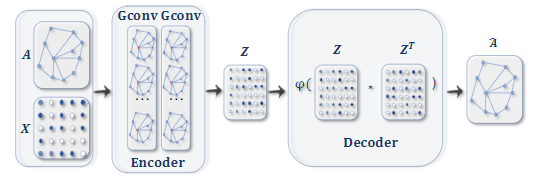
\includegraphics[width=14cm]{EdgeConv/main}
    \caption{基于邻边的图卷积神经网络更新示意图\cite{wang_dynamic_2019}}
    \label{fig:EdgeConv/main}
\end{figure}

对于结点i的更新,需要从结点i周围的5个邻居建立到结点i的邻边。对于其中某一条邻边$E_{j,i}$,其两个端点分别具有各自的特征,将特征拼接到一起,然后经过邻边卷积的多层感知器计算,即可得到邻边特征更新后的结果$e_{ij}$如图中左侧所示。
更新结点i周围所有的邻边特征,然后计算其和值,就形成了结点i更新之后的特征,如图\ref{fig:EdgeConv/main}中右侧所示。

\section{基于邻边卷积网络的复合物筛选模型}
\label{section:EdgeConv:detail}
本节分别介绍基于邻边卷积单层更新的具体实现,以及基于该单层更新方法构建的蛋白质复合物评价模型,最后介绍复合物筛选模型的总体实现流程。

\subsection{基于邻边卷积单层更新}

在通常的图卷积过程中,结点A的特征为周围所有结点的特征和自生特征决定,可以采取平均值的计算方法,如公式\ref{equ:NormalGCNNodeFlow}所示。
\begin{equation}
    \label{equ:NormalGCNNodeFlow}
    f_a=\delta (\frac{\sum_{i = 1}^{n}f_i+f_a}{n+1})
\end{equation}
其中$f_a$代表A结点的特征,$f_i$代表A结点所有邻居的特征,$\delta$为信息汇聚之后的特征更新函数。

在基于邻边卷积的复合物预测方法中,结点特征更新由其邻边共同决定。其具体计算过程如公式\ref{equ:EdgetoNodeFeat}所示。
\begin{equation}
    \label{equ:EdgetoNodeFeat}
    f_a=\delta (\frac{\sum_{i = 1}^{n}f_{ia}}{n})
\end{equation}
其中$f_{ia}$表示所有连接到A的邻边特征。其具体的汇聚过程如图\ref{fig:edge-feat-flow}所示,A结点汇聚周围所有邻边特征,包括$F_{BA}$、$F_{CA}$、$F_{DA}$以及$F_{EA}$。

\begin{figure}[htbp]
    \centering
    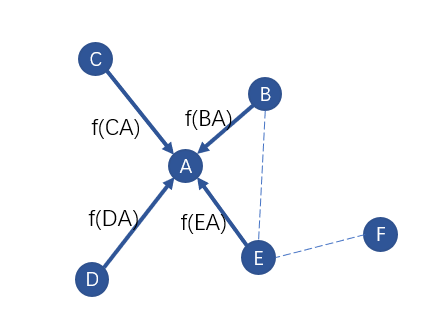
\includegraphics[width=7cm]{edge-feat-flow}
    \caption{边特征初始化结点特征示意图}
    \label{fig:edge-feat-flow}
\end{figure}

蛋白质生物数据是基于邻边的数据,因此在对复合物子图做图卷积的时候,基于生物特征的模型采用了基于edge的GCN模型\cite{wang_dynamic_2019},其具体的邻边更新方式如式\ref{equ:EdgeConv}所示。
\begin{equation}
    \label{equ:EdgeConv}
    h_i^{(l+1)} = \max_{j \in \mathcal{N}(i)} \mathrm{LeakyReLU}(
    \Theta \cdot (h_j^{(l)} - h_i^{(l)}) + \Phi \cdot h_i^{(l)})
\end{equation}
其中$h_i^{(l+1)}$表示第$l+1$层更新之后的结点数据,$h_j^{(l)} - h_i^{(l)}$表示从邻居结点到$i$结点的数据流,$h_i^{(l)}$为结点保留信息,$\Theta$和$\Phi$分别对应更新函数。$LeakyRelu$为激活函数。

每一轮基于edgeConv的卷积过程可以如下所示,首先是由结点更新邻边特征的过程,如图中上半部分所示,然后是用更新之后的邻边特征聚合物新的结点特征,如图中下半部分所示。

\begin{figure}[htbp]
    \centering
    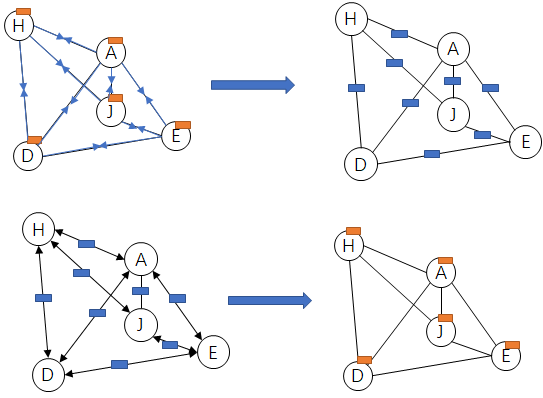
\includegraphics[width=10cm]{EdgeConv/edgeconv}
    \caption{总体EdgeConv图卷积过程示意图}
    \label{fig:EdgeConv/edgeconv}
\end{figure}

\subsection{特征子图评价模型}

本文处理了大量的生物学数据,包括蛋白质功能注释数据、结构域相互作用数据、亚细胞定位数据等,应用相关的生物领域的处理方法将生物学数据转换为可应用的特征数据,最终得到了11维度的特征数据。所有的特征都描述蛋白质相互作用,因此在图结构中,这些特征编码为图结构邻边的特征。
基于邻边卷积特征的复合物筛选模型总体流程如图\ref{fig:EdgeConv/flow}所示。

第一阶段如标号1所示,需要将初始的邻边特征以汇聚方法初始化结点特征,如图中上半部分所示。该汇聚方法为初始结点特征由其周围所有邻边特征的平均值替代。其具体的计算过程如公式\ref{equ:EdgetoNodeFeat}所示,其中激活函数为直接映射。其过程可被视为聚合阶段的基于边卷积神经网络过程,如图中\ref{fig:EdgeConv/edgeconv}下半部分所示。

第二阶段如标号2所示,需要基于邻边卷积将特征与拓扑结构融合,基于pool方法得到子图结构的特征表示,并基于子图特征做分类预测以及评分预测。其具体过程如图中下半部分所示。

模型使用了两层的基于邻边卷积的图神经网络,图卷积过程中隐层维度设置为64朴维。
两层图卷积之后,采用了对结点特征分别做最大值池化和平均值池化的方法,拼接到一起得到128维的子图特征。后续分别为两层感知器和softmax层得到图的分类预测,两层感知器和sigmoid层得到图的评分预测。


\begin{figure}[htbp]
    \centering
    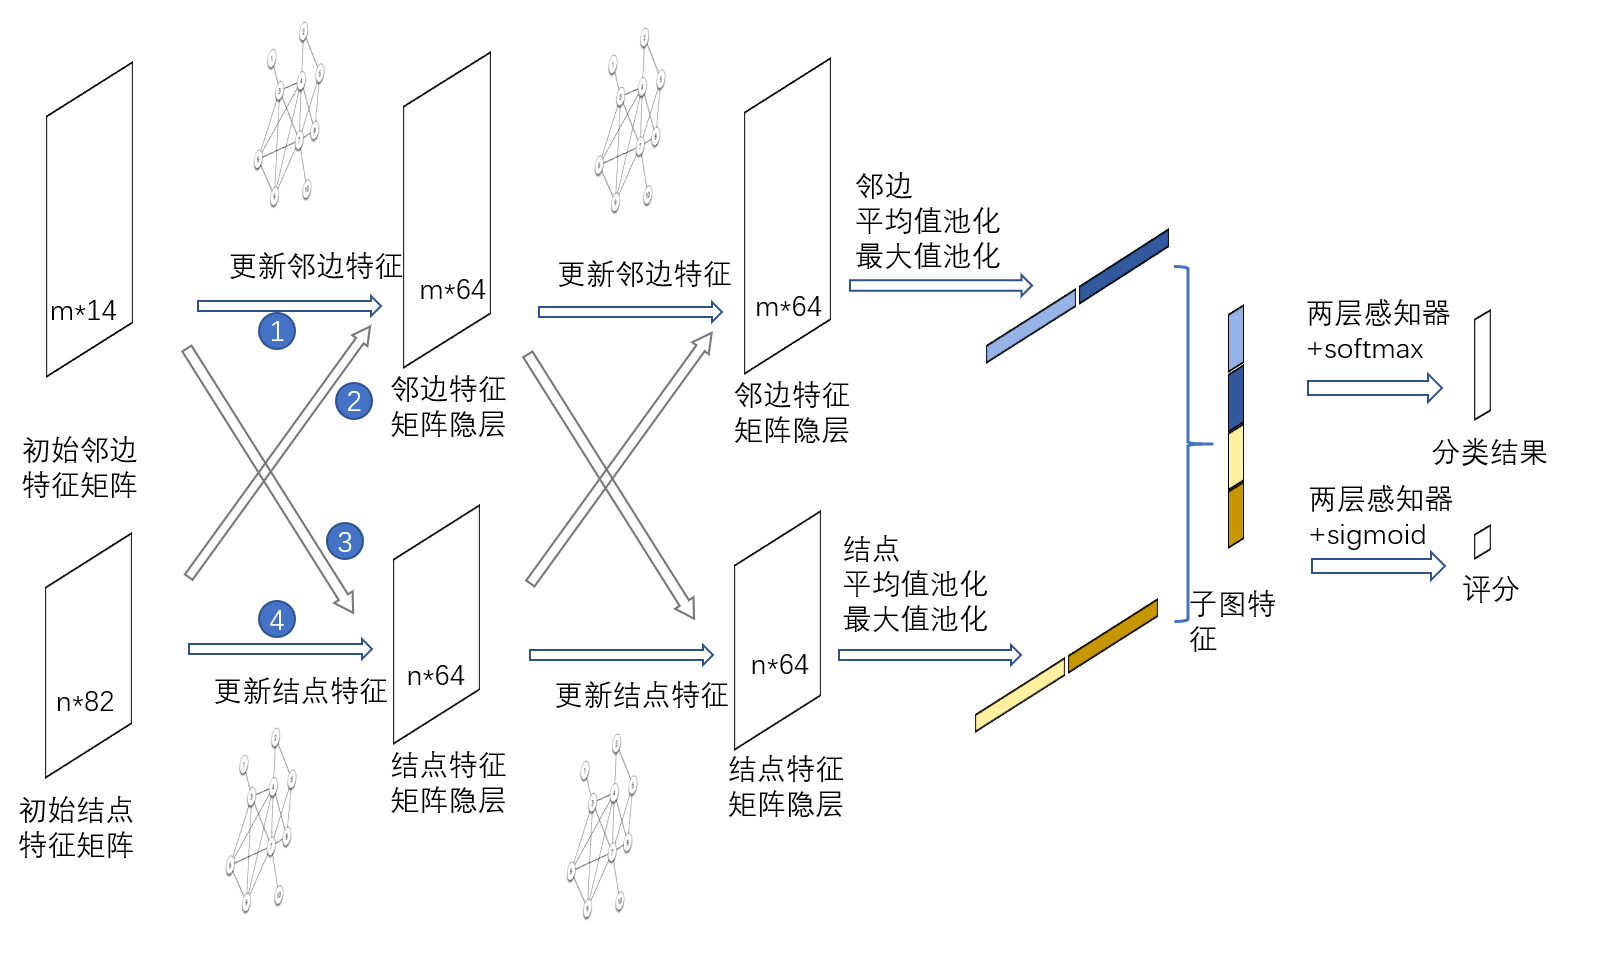
\includegraphics[width=16cm]{EdgeConv/flow}
    \caption{基于邻边卷积特征的复合物筛选模型总体流程}
    \label{fig:EdgeConv/flow}
\end{figure}

\subsection{筛选模型算法}
本节介绍基于邻边卷积的复合物筛选模型的具体算法,包括数据处理,模型训练,样本筛选与结果比对。
具体如算法\ref{alg:edgegcn-screen}所示。

\begin{algorithm}[h]
    \caption{Protein complex screening model based on edge convolution} % 名称
    \label{alg:edgegcn-screen}
    \begin{algorithmic}[1]
        \Require
        $Com_t$: train protein complexes;
        $Com_b$: protein complexes before screen;
        $Com_g$: golden bench protein complexes;
        $G$: protein-protein interaction network
        \Ensure
        $F1_a,F1_b/SPA_a,SPA_b$: predicted protein complexes F1/SPA metrix after and before screen;
        \State $n$:PIN node number;$m$:PIN edge number;$Com_a=None$;
        \State $F_{GO}\in \mathbb{R}^{m\times 2},F_{DDI}\in \mathbb{R}^{m\times 7},F_{Subcell}\in \mathbb{R}^{m\times 2},F_{Topo}\in \mathbb{R}^{m\times 1}$;
        \State $F_{E} \in \mathbb{R}^{m\times 12}=Concat(F_{GO},F_{DDI},F_{Subcell},F_{Topo})$;
        \State $Subs_t=Ext(G,F_{E},Com_t)$: feated subgraph extract algorithm;
        \For{i=0;i<epoch;i++}
        \For{$BSub_t \in Sub_t$} $loss=0$;
        \For{$Sub_t \in BSub_t$}
        \State $F_{N}^0 =MLP_m(Mean(Neighbor(F_{E}))), \in \mathbb{R}^{m\times 12}$;
        \State $F_{N}^1=EdgeConv(G,F_{N}^0), \in \mathbb{R}^{m\times 64}$
        \State $F_{N}^2=EdgeConv(G,F_{N}^1), \in \mathbb{R}^{m\times 64}$
        \State $F_t=Concat(MeanP(F_{N}^2),Maxp(F_{N}^2)), \in \mathbb{R}^{m\times 128}$;
        \State $PredC_t=MLP_C(F_t),\in \mathbb{R}^{1\times 4}$;$PredS_t=MLP_S(F_t),\in \mathbb{R}^{1}$;
        \State $loss+=\{CEL(PredC_t,LabelC_t)+\alpha \cdot BCEL(PredS_t,LabelS_t)\}$
        \EndFor; optimization $Adam(loss)$;
        \EndFor
        \EndFor
        \State $Subs_b=Ext(G,F_{E},Com_b)$: feated subgraph extract algorithm, see in \ref{section:featSubNetworkConstruct:allSample};
        \For{$Sub_b \in Subs_b$} $PredC_b=MLP_C(F_b)$;$PredS_b=MLP_S(F_b)$;
        \State $Com_a+=Complex(Sub_b)~if~PredC_b=positive|PredS_b>=0.25$;
        \EndFor
        \State $F1_a=F1(Com_a,Com_g),F1_b=F1(Com_b,Com_g)$;
        \State $SPA_a=SPA(Com_a,Com_g),SPA_b=SPA(Com_b,Com_g)$;
    \end{algorithmic}
\end{algorithm}
\section{实验设计及结果分析}
\label{section:EdgeConv:experience}

为了验证生物特征的添加对算法模型的提升,本文对比了在不添加生物数据,而使用相同的GCN结构的情况下,复合物分类模型对样本质量的提升程度。实验在DIP和Biogrid网络中分别运行了Dpclus、Clique和IPCA三个复合物生成算法。实验结果如下所示。
\begin{figure}[htbp]
    \centering
    \subcaptionbox{F1值对比}{\label{fig:result/DIP/F1/edge}
        \includegraphics[width=10cm]{result/DIP/F1/edge}}
    \vskip0.2cm
    \subcaptionbox{SPA值对比}{\label{fig:result/DIP/SPA/edge}
        \includegraphics[width=10cm]{result/DIP/SPA/edge}}
    \caption{DIP网络不同模型处理后结果对比}
    \label{fig:result/DIP/edge}
\end{figure}

\subparagraph*{实验方案(一)} ~

图\ref{fig:result/DIP/edge}为在DIP网络中,随机特征模型和基于生物特征的模型筛选之后结果的对比。
从图中可以看出,添加了生物特征后,在DIP网络中复合物的生成质量得到了相应的提升,同样的由于CLique算法的特征,该算法的前后对比提升幅度最为明显。

\subparagraph*{实验方案(二)} ~

图\ref{fig:result/Biogrid/edge}为在Biogrid网络中,随机特征模型和基于生物特征的模型筛选之后结果的对比。
\begin{figure}[htbp]
    \centering
    \subcaptionbox{F1值对比}{\label{fig:result/Biogrid/F1/edge}
        \includegraphics[width=10cm]{result/Biogrid/F1/edge}}
    \vskip0.2cm
    \subcaptionbox{SPA值对比}{\label{fig:result/Biogrid/SPA/edge}
        \includegraphics[width=10cm]{result/Biogrid/SPA/edge}}
    \caption{Biogrid网络不同模型处理后结果对比}
    \label{fig:result/Biogrid/edge}
\end{figure}
从图\ref{fig:result/Biogrid/edge}中可以看出添加了生物特征后,Biogrid网络相应样本的F1值均有较为明显的提升,而Clique算法的样本提升最为明显。综合评价指标SPA值也具有一定的提升。

图\ref{fig:result/DIP/edge}和图\ref{fig:result/Biogrid/edge}的数据如下所示。
\begin{table}[h]
    \centering
    \caption{DIP网络不同模型处理后结果对比数据}
    \begin{tabular}{C{2cm}C{2cm}C{2cm}C{2cm}}
        \toprule
        \textbf{F1值} & \textbf{原始数据} & \textbf{随机GCN筛选} &\textbf{邻边特征GCN筛选} \\
        \midrule
        Dpclus算法    & 0.414             & 0.352                & 0.484                                 \\
        Clique算法    & 0.296             & 0.222                & 0.453                              \\
        IPCA算法      & 0.291             & 0.300                & 0.420                               \\
        \bottomrule
    \end{tabular}
    \begin{tabular}{C{2cm}C{2cm}C{2cm}C{2cm}}
        \toprule
        \textbf{SPA值} & \textbf{原始数据} & \textbf{随机GCN筛选} & \textbf{邻边特征GCN筛选} \\
        \midrule
        Dpclus算法     & 1.333             & 1.340                & 1.490                                    \\
        Clique算法     & 0.658             & 0.596                & 0.731                                  \\
        IPCA算法       & 0.794             & 0.729                & 0.838                               \\
        \bottomrule
    \end{tabular}
\end{table}

\begin{table}[h]
    \centering
    \caption{Biogrid网络不同模型处理后结果对比数据}
    \begin{tabular}{C{2cm}C{2cm}C{2cm}C{2cm}}
        \toprule
        \textbf{F1值} & \textbf{原始数据} & \textbf{随机GCN筛选} &\textbf{邻边特征GCN筛选} \\
        \midrule
        Dpclus算法    & 0.425             & 0.445                & 0.529                                 \\
        Clique算法    & 0.203             & 0.216                & 0.510                              \\
        IPCA算法      & 0.294             & 0.122                & 0.373                               \\
        \bottomrule
    \end{tabular}
    \begin{tabular}{C{2cm}C{2cm}C{2cm}C{2cm}}
        \toprule
        \textbf{SPA值} & \textbf{原始数据} & \textbf{随机GCN筛选} & \textbf{邻边特征GCN筛选} \\
        \midrule
        Dpclus算法     & 1.796             & 1.119                & 1.950                                    \\
        Clique算法     & 0.901             & 0.532                & 1.011                                  \\
        IPCA算法       & 0.859             & 0.886                & 0.891                               \\
        \bottomrule
    \end{tabular}
\end{table}


\section{本章小结}
\label{section:EdgeConv:summary}

本章基于特征子图中的邻边相似性出发,探讨了仅仅使用生物特征转换为的邻边数据的基础上,复合物筛选模型可达到的效果提升。提出了使用基于邻边卷积的图神经网络方法以及相应的模型,阐述了邻边特征如何初始化结点特征,以及EdgeConv的信息流更新过程。最后本章对比了基础的无特征EdgeConv模型,并进行了实验,实验结果表明了生物特征的有效性以及邻边卷积能较好的处理生物相似性数据。